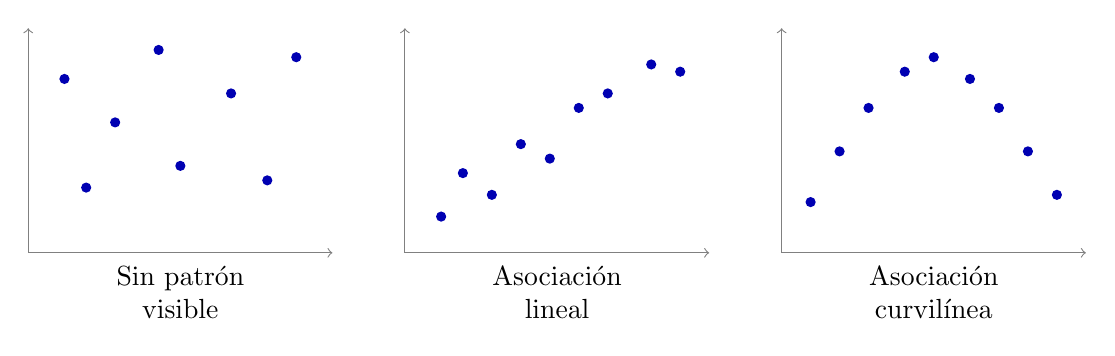
\begin{tikzpicture}[scale=0.92]
    % Sin patrón evidente
    \begin{scope}
        \draw[->,gray] (0,0) -- (4.2,0);
        \draw[->,gray] (0,0) -- (0,3.1);
        \foreach \x/\y in {0.5/2.4,0.8/0.9,1.2/1.8,1.8/2.8,2.1/1.2,2.8/2.2,3.3/1.0,3.7/2.7} {\fill[blue!70!black] (\x,\y) circle (2pt);}
        \node[align=center] at (2.1,-0.55) {Sin patrón\\visible};
    \end{scope}
    % Asociación estadística lineal
    \begin{scope}[xshift=5.2cm]
        \draw[->,gray] (0,0) -- (4.2,0);
        \draw[->,gray] (0,0) -- (0,3.1);
        \foreach \x/\y in {0.5/0.5,0.8/1.1,1.2/0.8,1.6/1.5,2.0/1.3,2.4/2.0,2.8/2.2,3.4/2.6,3.8/2.5} {\fill[blue!70!black] (\x,\y) circle (2pt);}
        \node[align=center] at (2.1,-0.55) {Asociación\\lineal};
    \end{scope}
    % Asociación estadística curvilínea
    \begin{scope}[xshift=10.4cm]
        \draw[->,gray] (0,0) -- (4.2,0);
        \draw[->,gray] (0,0) -- (0,3.1);
        \foreach \x/\y in {0.4/0.7,0.8/1.4,1.2/2.0,1.7/2.5,2.1/2.7,2.6/2.4,3.0/2.0,3.4/1.4,3.8/0.8} {\fill[blue!70!black] (\x,\y) circle (2pt);}
        \node[align=center] at (2.1,-0.55) {Asociación\\curvilínea};
    \end{scope}
\end{tikzpicture}